\documentclass[oneside]{book}

\usepackage{amsmath, amsthm, amssymb, amsfonts}
\usepackage{thmtools}
\usepackage{graphicx}
\usepackage{setspace}
\usepackage{geometry}
\usepackage{float}
\usepackage{hyperref}
\usepackage[utf8]{inputenc}
\usepackage[english]{babel}
\usepackage{framed}
\usepackage[dvipsnames]{xcolor}
\usepackage{environ}
\usepackage{tcolorbox}
\tcbuselibrary{theorems,skins,breakable}

\setstretch{1.2}
\geometry{
    textheight=9in,
    textwidth=5.5in,
    top=1in,
    headheight=12pt,
    headsep=25pt,
    footskip=30pt
}

% Variables
\def\notetitle{MATH 165\\Linear Algebra \& Diff. Equation\\Midterm II \\Review Note with Examples}
\def\noteauthor{
    \textbf{Professor Madhu} \\ 
    {\LaTeX} by Ethan\\
    University of Rochester}
\def\notedate{Spring 2024}

% The theorem system and user-defined commands
% Theorem System
% The following boxes are provided:
%   Definition:     \defn 
%   Theorem:        \thm 
%   Lemma:          \lem
%   Corollary:      \cor
%   Proposition:    \prop   
%   Claim:          \clm
%   Fact:           \fact
%   Proof:          \pf
%   Example:        \ex
%   Remark:         \rmk (sentence), \rmkb (block)
% Suffix
%   r:              Allow Theorem/Definition to be referenced, e.g. thmr
%   p:              Add a short proof block for Lemma, Corollary, Proposition or Claim, e.g. lemp
%                   For theorems, use \pf for proof blocks

% Definition
\newtcbtheorem[number within=section]{mydefinition}{Definition}
{
    enhanced,
    frame hidden,
    titlerule=0mm,
    toptitle=1mm,
    bottomtitle=1mm,
    fonttitle=\bfseries\large,
    coltitle=black,
    colbacktitle=green!20!white,
    colback=green!10!white,
}{defn}

\NewDocumentCommand{\defn}{m+m}{
    \begin{mydefinition}{#1}{}
        #2
    \end{mydefinition}
}

\NewDocumentCommand{\defnr}{mm+m}{
    \begin{mydefinition}{#1}{#2}
        #3
    \end{mydefinition}
}

% Theorem
\newtcbtheorem[use counter from=mydefinition]{mytheorem}{Theorem}
{
    enhanced,
    frame hidden,
    titlerule=0mm,
    toptitle=1mm,
    bottomtitle=1mm,
    fonttitle=\bfseries\large,
    coltitle=black,
    colbacktitle=cyan!20!white,
    colback=cyan!10!white,
}{thm}

\NewDocumentCommand{\thm}{m+m}{
    \begin{mytheorem}{#1}{}
        #2
    \end{mytheorem}
}

\NewDocumentCommand{\thmr}{mm+m}{
    \begin{mytheorem}{#1}{#2}
        #3
    \end{mytheorem}
}

% Lemma
\newtcbtheorem[use counter from=mydefinition]{mylemma}{Lemma}
{
    enhanced,
    frame hidden,
    titlerule=0mm,
    toptitle=1mm,
    bottomtitle=1mm,
    fonttitle=\bfseries\large,
    coltitle=black,
    colbacktitle=violet!20!white,
    colback=violet!10!white,
}{lem}

\NewDocumentCommand{\lem}{m+m}{
    \begin{mylemma}{#1}{}
        #2
    \end{mylemma}
}

\newenvironment{lempf}{
	{\noindent{\it \textbf{Proof for Lemma}}}
	\tcolorbox[blanker,breakable,left=5mm,parbox=false,
    before upper={\parindent15pt},
    after skip=10pt,
	borderline west={1mm}{0pt}{violet!20!white}]
}{
    \textcolor{violet!20!white}{\hbox{}\nobreak\hfill$\blacksquare$} 
    \endtcolorbox
}

\NewDocumentCommand{\lemp}{m+m+m}{
    \begin{mylemma}{#1}{}
        #2
    \end{mylemma}

    \begin{lempf}
        #3
    \end{lempf}
}

% Corollary
\newtcbtheorem[use counter from=mydefinition]{mycorollary}{Corollary}
{
    enhanced,
    frame hidden,
    titlerule=0mm,
    toptitle=1mm,
    bottomtitle=1mm,
    fonttitle=\bfseries\large,
    coltitle=black,
    colbacktitle=orange!20!white,
    colback=orange!10!white,
}{cor}

\NewDocumentCommand{\cor}{+m}{
    \begin{mycorollary}{}{}
        #1
    \end{mycorollary}
}

\newenvironment{corpf}{
	{\noindent{\it \textbf{Proof for Corollary.}}}
	\tcolorbox[blanker,breakable,left=5mm,parbox=false,
    before upper={\parindent15pt},
    after skip=10pt,
	borderline west={1mm}{0pt}{orange!20!white}]
}{
    \textcolor{orange!20!white}{\hbox{}\nobreak\hfill$\blacksquare$} 
    \endtcolorbox
}

\NewDocumentCommand{\corp}{m+m+m}{
    \begin{mycorollary}{}{}
        #1
    \end{mycorollary}

    \begin{corpf}
        #2
    \end{corpf}
}

% Proposition
\newtcbtheorem[use counter from=mydefinition]{myproposition}{Proposition}
{
    enhanced,
    frame hidden,
    titlerule=0mm,
    toptitle=1mm,
    bottomtitle=1mm,
    fonttitle=\bfseries\large,
    coltitle=black,
    colbacktitle=yellow!30!white,
    colback=yellow!20!white,
}{prop}

\NewDocumentCommand{\prop}{+m}{
    \begin{myproposition}{}{}
        #1
    \end{myproposition}
}

\newenvironment{proppf}{
	{\noindent{\it \textbf{Proof for Proposition.}}}
	\tcolorbox[blanker,breakable,left=5mm,parbox=false,
    before upper={\parindent15pt},
    after skip=10pt,
	borderline west={1mm}{0pt}{yellow!30!white}]
}{
    \textcolor{yellow!30!white}{\hbox{}\nobreak\hfill$\blacksquare$} 
    \endtcolorbox
}

\NewDocumentCommand{\propp}{+m+m}{
    \begin{myproposition}{}{}
        #1
    \end{myproposition}

    \begin{proppf}
        #2
    \end{proppf}
}

% Claim
\newtcbtheorem[use counter from=mydefinition]{myclaim}{Claim}
{
    enhanced,
    frame hidden,
    titlerule=0mm,
    toptitle=1mm,
    bottomtitle=1mm,
    fonttitle=\bfseries\large,
    coltitle=black,
    colbacktitle=pink!30!white,
    colback=pink!20!white,
}{clm}


\NewDocumentCommand{\clm}{m+m}{
    \begin{myclaim*}{#1}{}
        #2
    \end{myclaim*}
}

\newenvironment{clmpf}{
	{\noindent{\it \textbf{Proof for Claim.}}}
	\tcolorbox[blanker,breakable,left=5mm,parbox=false,
    before upper={\parindent15pt},
    after skip=10pt,
	borderline west={1mm}{0pt}{pink!30!white}]
}{
    \textcolor{pink!30!white}{\hbox{}\nobreak\hfill$\blacksquare$} 
    \endtcolorbox
}

\NewDocumentCommand{\clmp}{m+m+m}{
    \begin{myclaim*}{#1}{}
        #2
    \end{myclaim*}

    \begin{clmpf}
        #3
    \end{clmpf}
}

% Fact
\newtcbtheorem[use counter from=mydefinition]{myfact}{Fact}
{
    enhanced,
    frame hidden,
    titlerule=0mm,
    toptitle=1mm,
    bottomtitle=1mm,
    fonttitle=\bfseries\large,
    coltitle=black,
    colbacktitle=purple!20!white,
    colback=purple!10!white,
}{fact}

\NewDocumentCommand{\fact}{+m}{
    \begin{myfact}{}{}
        #1
    \end{myfact}
}


% Proof
\NewDocumentCommand{\pf}{+m}{
    \begin{proof}
        [\noindent\textbf{Proof.}]
        #1
    \end{proof}
}

% Example
\newenvironment{example}{%
    \par
    \vspace{5pt}
	\begin{minipage}{\textwidth}
		\noindent\textbf{Example.}
		\tcolorbox[blanker,breakable,left=5mm,parbox=false,
	    before upper={\parindent15pt},
	    after skip=10pt,
		borderline west={1mm}{0pt}{cyan!10!white}]
}{%
		\endtcolorbox
	\end{minipage}
    \vspace{5pt}
}

\NewDocumentCommand{\ex}{+m}{
    \begin{example}
        #1
    \end{example}
}


% Remark
\NewDocumentCommand{\rmk}{+m}{
    {\it \color{blue!50!white}#1}
}

\newenvironment{remark}{
    \par
    \vspace{5pt}
    \begin{minipage}{\textwidth}
        {\par\noindent{\textbf{Remark.}}}
        \tcolorbox[blanker,breakable,left=5mm,
        before skip=10pt,after skip=10pt,
        borderline west={1mm}{0pt}{cyan!10!white}]
}{
        \endtcolorbox
    \end{minipage}
    \vspace{5pt}
}

\NewDocumentCommand{\rmkb}{+m}{
    \begin{remark}
        #1
    \end{remark}
}


\newcommand{\lcm}{\operatorname{lcm}}



% ------------------------------------------------------------------------------

\begin{document}
\title{\textbf{
    \LARGE{\notetitle} \vspace*{10\baselineskip}}
    }
\author{\noteauthor}
\date{\notedate}

\maketitle
\newpage

\tableofcontents
\newpage

% ------------------------------------------------------------------------------
\chapter{Determinants}
\section{Lecture 9: Def. of Determinants \& it's calculation}

\rmk{
    This lecture covers: 
    % \\ - 3.1 The Definition of the Determinant\\- 3.3 Cofactor Expansions (partly)
    \begin{itemize}
        \item 3.1 The Definition of the Determinant
        \item 3.3 Cofactor Expansions (partly)
    \end{itemize}
}

\subsection{What is Determinanrts}

\defn{Determinants}{
    The \textbf{determinants} of a square matrix $A$, denoted $\det{(A)}$, is a number associated with the matrix $A$ that is \textit{designed} to carry information about the invertibility (among other things) of the matrix $A$. We also use the notation $|A|$ to denote the determinant of $A$. 
}
The way we calculate determinants is derived from the fact of changing the matrix into RREF (Reduce-Row-Echelon-Form) and seeing if the matrix is invertible. If the matrix is invertible, then the determinant is not zero. If the matrix is not invertible, then the determinant is zero. The way we calculate it is based on observation. (P.196)

\subsection{How to calculate Determinants}
\paragraph{1 by 1 matrix}

The determinant of a $1 \times 1$ matrix $[a11]$ is $a_{11}$. 

\ex{
    \\
    \textbf{Calculate the determinant of the matrix $A = [3]$. }
    \[
        \begin{vmatrix}
            3
        \end{vmatrix} = 3
    \]
    \textbf{What is the rank of the matrix $A$? } \\The rank of the matrix $A$ is 1.

}
\\\\
\ex{
    \\
    \textbf{Calculate the determinant of the matrix $A = [0]$. }\\
    \[
        \begin{vmatrix}
            0
        \end{vmatrix} = 0
    \]
    \textbf{What is the rank of the matrix $A$? } \\
    The rank of the matrix $A$ is 0. (Since the determinant is 0, the matrix is not invertible.)

}


\paragraph{2 by 2 matrix} 

The determinant of a $2 \times 2$ matrix $A = \begin{bmatrix} a & b \\ c & d \end{bmatrix}$ is given by $ad=bc$. 
\[
    \begin{vmatrix}
        a & b \\
        c & d
    \end{vmatrix} 
    = ad - bc
\]

The way we calculate it is by taking the product of the diagonal elements and subtracting the product of the off-diagonal elements.


\ex{
    \textbf{Calculate the determinant of the matrix $A = \begin{bmatrix} 1 & 2 \\ 3 & 4 \end{bmatrix}$. }
    \[
        \begin{vmatrix}
            1 & 2 \\
            3 & 4
        \end{vmatrix} = 1 \cdot 4 - 2 \cdot 3 = 4 - 6 = -2
    \]
    \textbf{What is the rank of the matrix $A$? } \\The rank of the matrix $A$ is 2.\\
    \textbf{Is the matrix invertible? } \\Yes, the matrix is invertible, since $-2 \neq 0$.
}

\ex{
    \textbf{Calculate the determinant of the matrix $A = \begin{bmatrix} 2 & 3 \\ 4 & 6 \end{bmatrix}$. }
    \[
        \begin{vmatrix}
            2 & 3 \\
            4 & 6
        \end{vmatrix} = 2 \cdot 6 - 3 \cdot 4 = 12 - 12 = 0
    \]
    \textbf{What is the rank of the matrix $A$? } \\The rank of the matrix $A$ is 1.\\
    \textbf{Is the matrix invertible? } \\No, the matrix is not invertible, since $0 = 0$.
}



\paragraph{3 by 3 matrix}
The determinant of a $ 3 \times 3 $ matrixhas a similar 'diagonals'-type definition:
\[
    |A|= \begin{vmatrix}
        a & b & c \\
        d & e & f \\
        g & h & i
    \end{vmatrix}
    = aei + bfg + cdh - ceg - bdi - afh
\]


We can use a clever trick with arrows by repeating the first two columns to calculate the determinant of a $3 \times 3$ matrix.



\begin{figure}
    \begin{center}
        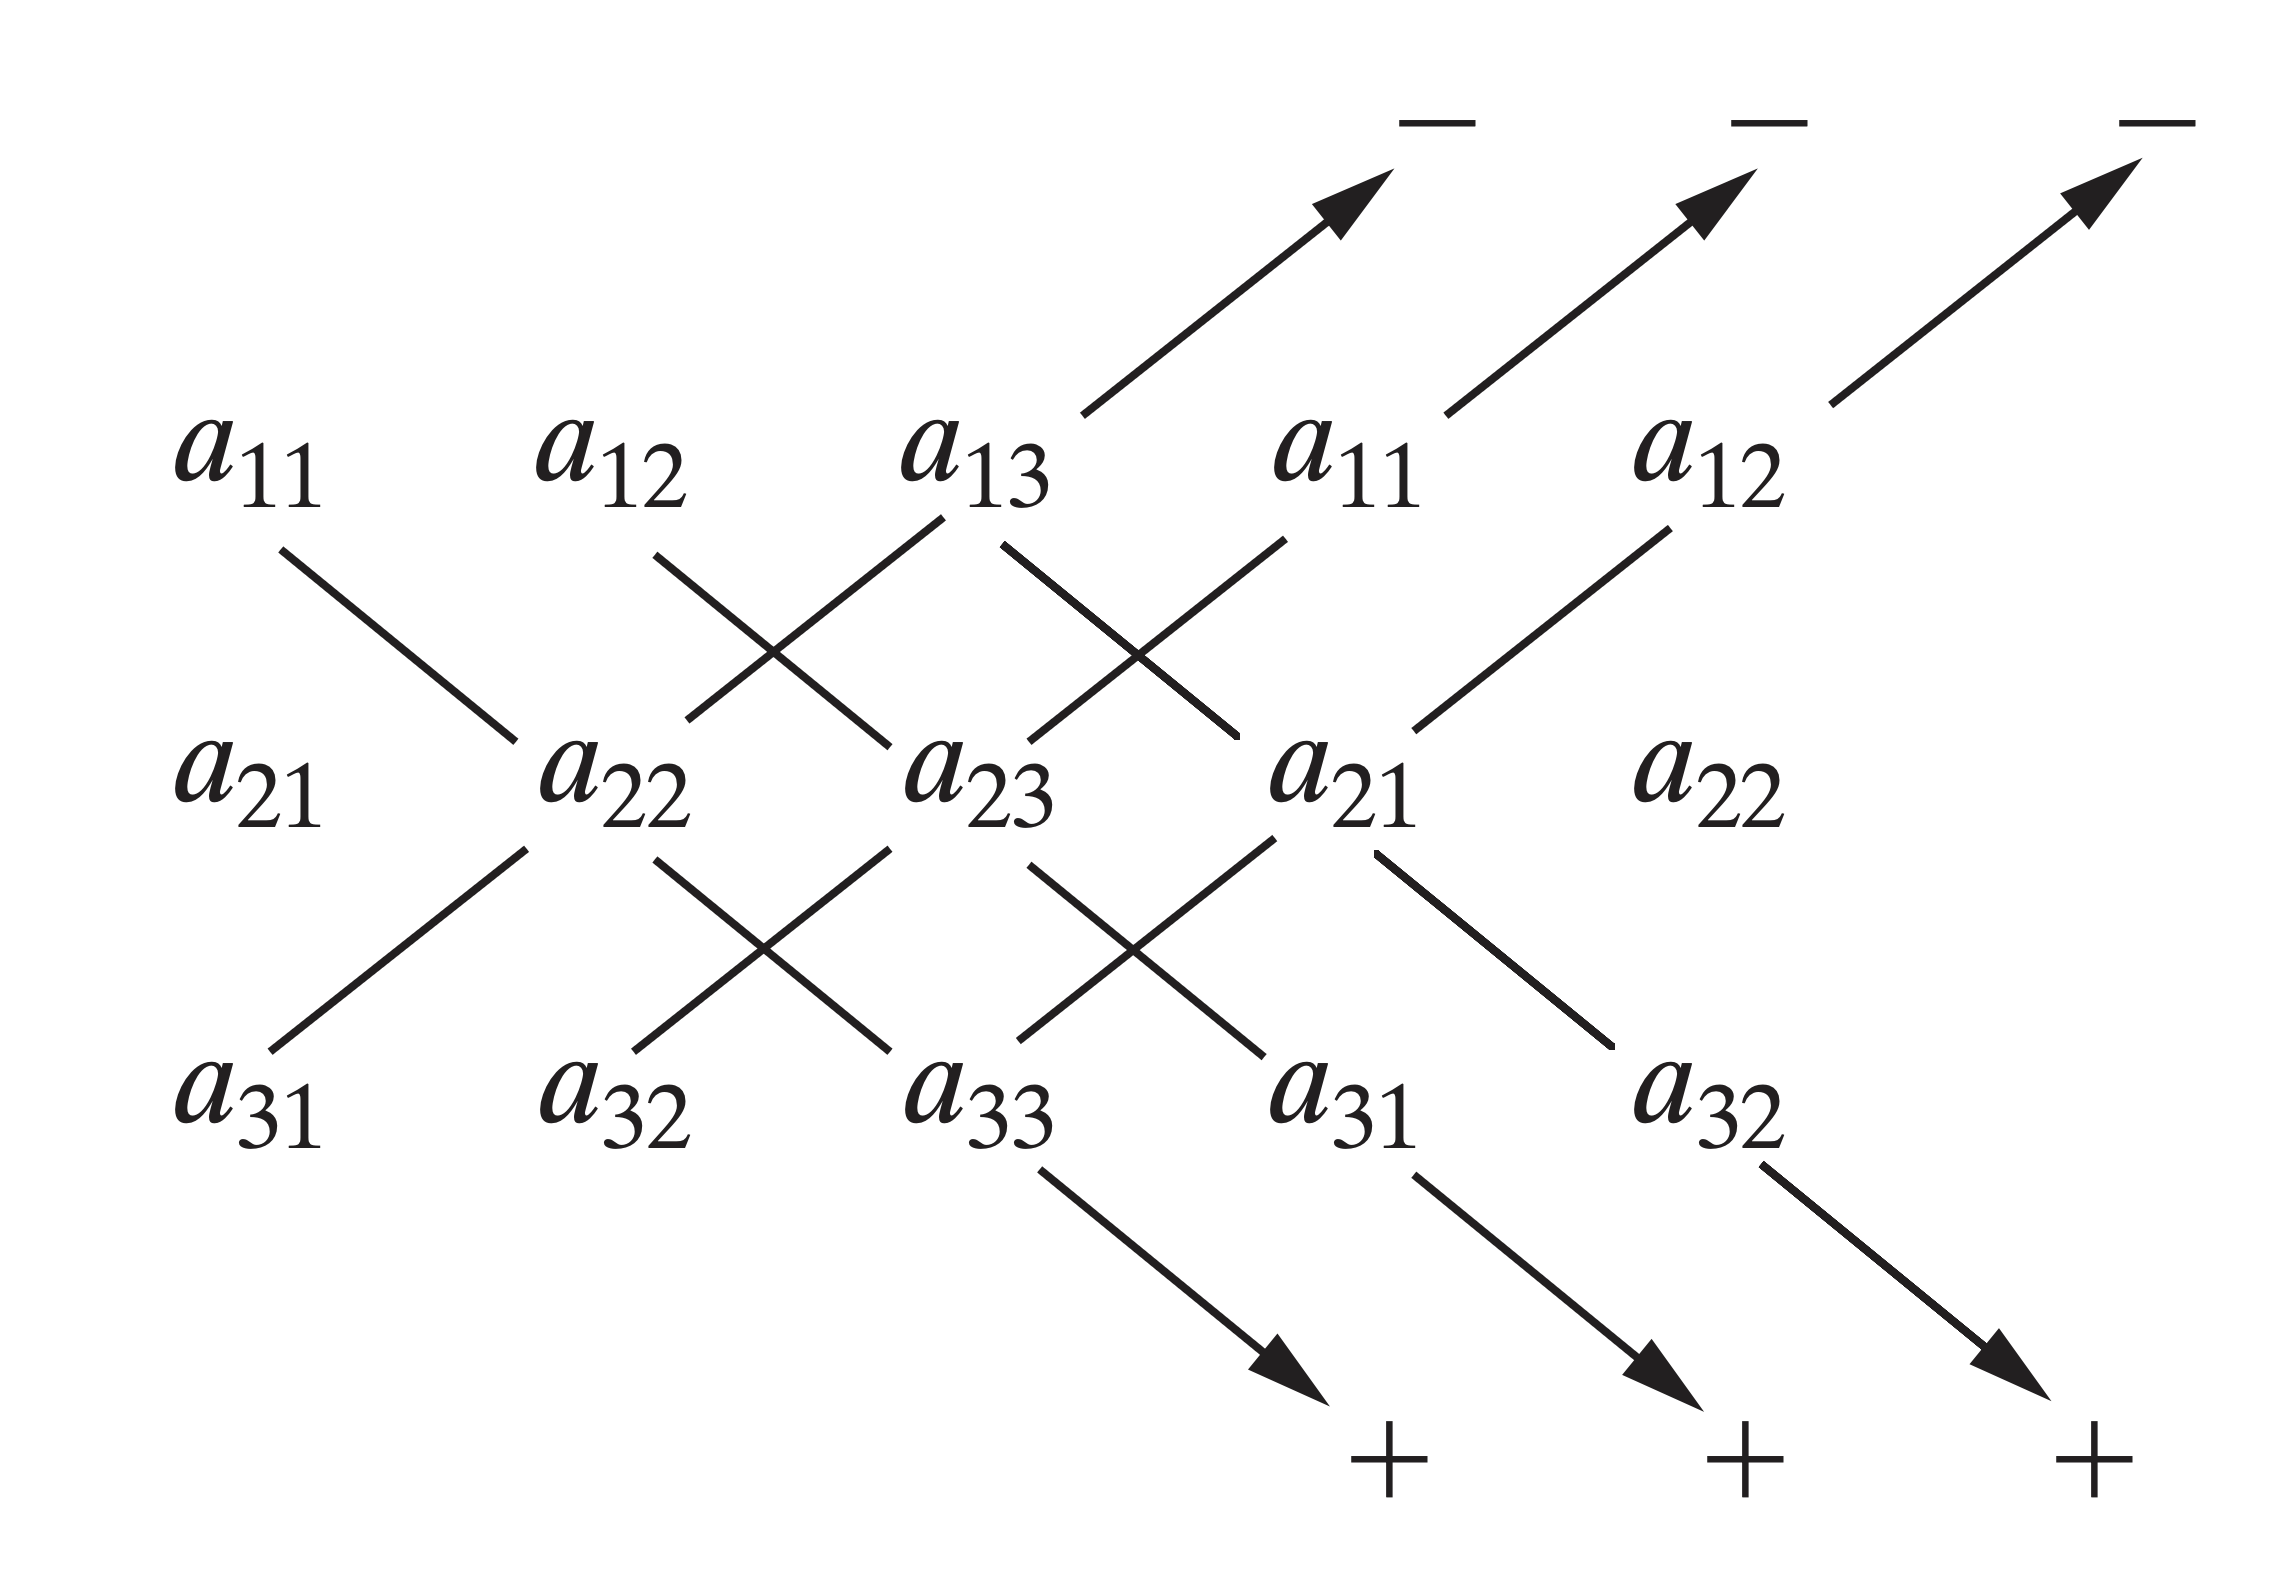
\includegraphics[scale=0.1]{img/Snipaste_2024-03-27_13-52-06.png}
        \caption{Determinant of a $3 \times 3$ matrix}
    \end{center}
\end{figure}





\ex{
    \textbf{Calculate the determinant of the matrix $A = \begin{bmatrix} 1 & 2 & 3 \\ 4 & 5 & 6 \\ 7 & 8 & 9 \end{bmatrix}$. }
    \[
        \begin{vmatrix}
            1 & 2 & 3 \\
            4 & 5 & 6 \\
            7 & 8 & 9
        \end{vmatrix} = 1 \cdot 5 \cdot 9 + 2 \cdot 6 \cdot 7 + 3 \cdot 4 \cdot 8 - 3 \cdot 5 \cdot 7 - 2 \cdot 4 \cdot 9 - 1 \cdot 6 \cdot 8 = 0
    \]
    \textbf{What is the rank of the matrix $A$? } \\The rank of the matrix $A$ is 2.\\
    \textbf{Is the matrix invertible? } \\No, the matrix is not invertible, since $0 = 0$.

}


\rmkb{
    If the dimension of a matrix is greater than $3 \times 3$, we won’t be able to find the determinant in one step, as the sub-matrices will have dimension at least $3 \times 3$.
}


\paragraph{Larger matrix}

Another more common way to find the determinant of a $3 \times 3$ matrix is to use the \textbf{cofactor expansion} method. The cofactor expansion method is a way to calculate the determinant of a matrix by breaking it down into smaller matrices. This can also apply to \textbf{larger matrices}.
\[
    \begin{vmatrix}
        a & b & c \\
        d & e & f \\
        g & h & i
    \end{vmatrix} 
    = a \begin{vmatrix}
        e & f \\
        h & i
    \end{vmatrix} - b \begin{vmatrix}
        d & f \\
        g & i
    \end{vmatrix} + c \begin{vmatrix}
        d & e \\
        g & h
    \end{vmatrix}
\]

\thmr{Cofactor Expansion}{}{
    We may expandalong row $i$:

    \[
        \det(A) = a_{i1}C_{i1} + a_{i2}C_{i2} + \cdots + a_{in}C_{in} = \sum_{j=1}^{n} a_{ij}C_{ij}
    \]


    We may expand along column $j$:

    \[
        \det(A) = a_{1j}C_{1j} + a_{2j}C_{2j} + \cdots + a_{nj}C_{nj} = \sum_{i=1}^{n} a_{ij}C_{ij}
    \]

}


The way you do so is to choose a row or a column (typically, a row or column with the most zeros) and expand the determinant along that row or column. If the matrix after expansion is still not a $2 \times 2$ matrix, you can expand it again.



\ex{\\
    \textbf{Calculate the determinant of the matrix $A = \begin{bmatrix} 1 & 2 & 3 & 4 \\ 5 & 6 & 7 & 8 \\ 9 & 10 & 11 & 12 \\ 13 & 14 & 15 & 16 \end{bmatrix}$. }\\\\\\
    Let's choose the first row to expand the determinant.
    \[
        \begin{vmatrix}
            1 & 2 & 3 & 4 \\
            5 & 6 & 7 & 8 \\
            9 & 10 & 11 & 12 \\
            13 & 14 & 15 & 16
        \end{vmatrix} 
        = 1 \begin{vmatrix}
            6 & 7 & 8 \\
            10 & 11 & 12 \\
            14 & 15 & 16
        \end{vmatrix} - 2 \begin{vmatrix}
            5 & 7 & 8 \\
            9 & 11 & 12 \\
            13 & 15 & 16
        \end{vmatrix} + 3 \begin{vmatrix}
            5 & 6 & 8 \\
            9 & 10 & 12 \\
            13 & 14 & 16
        \end{vmatrix} - 4 \begin{vmatrix}
            5 & 6 & 7 \\
            9 & 10 & 11 \\
            13 & 14 & 15
        \end{vmatrix}
    \]
    % \\\\\\\\\\\\
    \[
        = 1 \times 6 \begin{vmatrix}
            11 & 12 \\
            15 & 16
        \end{vmatrix} - 2 \times 7 \begin{vmatrix}
            9 & 12 \\
            13 & 16
        \end{vmatrix} + 3 \times 8 \begin{vmatrix}
            9 & 11 \\
            13 & 15
        \end{vmatrix} - 4 \times 5 \begin{vmatrix}
            10 & 11 \\
            14 & 15
        \end{vmatrix} \text{...} = 0
    \]
    \\
    \textbf{What is the rank of the matrix $A$? } \\The rank of the matrix $A$ is 2.\\\\
    \textbf{Is the matrix invertible? } \\No, the matrix is not invertible, since $0 = 0$.\\
}

\subsection{Inverse of 2 by 2 matrix}

\prop{
    Let $A = \begin{bmatrix} a & b \\ c & d \end{bmatrix}$ be a $2 \times 2$ matrix. If $\det(A) \neq 0$, then the inverse of $A$ is given by
    \[
        A^{-1} = \frac{1}{\det(A)} \begin{bmatrix} d & -b \\ -c & a \end{bmatrix}
    \]

}
\pf{
    Let $A = \begin{bmatrix} a & b \\ c & d \end{bmatrix}$ be a $2 \times 2$ matrix. If $\det(A) \neq 0$, then
    \[
        A = \begin{pmatrix}
        a & b \\
        c & d
    \end{pmatrix}
    \]
    \[
        A^{-1} = \frac{1}{\det(A)} \begin{bmatrix} d & -b \\ -c & a \end{bmatrix}
    \]
    \[
        = \frac{1}{ad - bc} \begin{bmatrix} d & -b \\ -c & a \end{bmatrix}
    \]
    \[
        A \times A^{-1} = \begin{pmatrix}
        a & b \\
        c & d
        \end{pmatrix} \times \frac{1}{ad - bc} \begin{pmatrix}
        d & -b \\
        -c & a
        \end{pmatrix}
    \]
    \[
        \frac{1}{ad - bc}(a \times d + b \times (-c)) = \frac{ad - bc}{ad - bc} = 1
    \]
    \[
        \frac{1}{ad - bc}(a \times (-b) + b \times a) = \frac{-ab + ab}{ad - bc} = 0
    \]
    \[
        \frac{1}{ad - bc}(c \times d + d \times (-c)) = \frac{cd - cd}{ad - bc} = 0
    \]
    \[
        \frac{1}{ad - bc}(c \times (-b) + d \times a) = \frac{-bc + ad}{ad - bc} = 1
    \]
    \[
        A \times A^{-1}
        =
        \begin{pmatrix}
            1 & 0 \\
            0 & 1
        \end{pmatrix}
        = I
    \]

    Thus, $A^{-1} = \frac{1}{\det(A)} \begin{bmatrix} d & -b \\ -c & a \end{bmatrix}$.

}

\ex{
    \textbf{Find the inverse of the matrix $A = \begin{bmatrix} 1 & 2 \\ 3 & 4 \end{bmatrix}$. }
    \[
        \begin{vmatrix}
            1 & 2 \\
            3 & 4
        \end{vmatrix} = 1 \cdot 4 - 2 \cdot 3 = 4 - 6 = -2
    \]
    Since $\det(A) = -2 \neq 0$, we can find the inverse of $A$.
    \[
        A^{-1} = \frac{1}{-2} \begin{bmatrix} 4 & -2 \\ -3 & 1 \end{bmatrix} = \begin{bmatrix} -2 & 1 \\ 3/2 & -1/2 \end{bmatrix}
    \]

}




\subsection{Determinat of matrix functions}
Given a matrix function $M (t)$, its determinant $\det(M (t))$ can be found using exactly the same techniques as that of a numerical matrix. The only difference is that the determinant is a function of t.

\ex{
    \textbf{Find} \[
        \begin{vmatrix}
            \cos(t) & -\sin(t) \\
            \cos(t) & \sin(t)
        \end{vmatrix}
    \]

    \[
        \begin{vmatrix}
            \cos(t) & -\sin(t) \\
            \cos(t) & \sin(t)
        \end{vmatrix}
        = \cos(t) \cdot \sin(t) - (-\sin(t) \cdot \cos(t))
    \]
    \[
        = \sin(t) \cdot \cos(t) + \sin(t) \cdot \cos(t) 
    \]
    \[= 2 \sin(t) \cdot \cos(t)\]
    \[\boxed{= \sin(2t)} \]

}





\subsection{Geometry Application: areas and volumes}

\paragraph{Areas}
Suppose $O$ is the origin in the xy-plane. Let P be a parallelogram with vertices $O = (0, 0)$,$ A = (a_1, a_2)$, $B = (b_1, b_2)$, and $C = (c_1, c_2)$.

\fact{
    The area of the parallelogram P is given by
    \[
        \text{Area}(P) = \begin{vmatrix}
            \det \begin{pmatrix}
                \begin{bmatrix}
                    a_1 & a_2 \\
                    b_1 & b_2
                \end{bmatrix}
            \end{pmatrix}
        \end{vmatrix}
    \]
}
Since the area is always positive, we take the absolute value of the determinant.


\paragraph{Volumes}
Similarly, the volume of a parallelepiped in $\mathbb{R}^3$ is given by the absolute value of the determinant of the matrix whose rows are the vectors representing the edges of the parallelepiped.

\fact{
    The volume of the parallelepiped determined by sides $OA$, $OB$, and $OC$ where
    \[
        A=(a_1, a_2, a_3), B=(b_1, b_2, b_3), C=(c_1, c_2, c_3)
    \]
    is given by
    \[
        \text{Volume} = \begin{vmatrix}
            \det \begin{pmatrix}
                \begin{bmatrix}
                    a_1 & a_2 & a_3 \\
                    b_1 & b_2 & b_3 \\
                    c_1 & c_2 & c_3
                \end{bmatrix}
            \end{pmatrix}
        \end{vmatrix}
    \]

}


\pf{
    The area of the parallelogram is 
    Area = (length of base) $\times$ (perpendicular height).\\
    This can be written as \\
    \[
        \text{Area } = ||a||h = ||a||  ||b|| \space \sin(\theta) ||a \times b||
    \]
    Since the k components of a and b are both zero (since the vectors lie in thexy-plane), substitution from Equation yields
    \[
        \text{Area} = ||(a_1 b_2 - a_2 b_1)k|| = |a_1 b_2 - a_2 b_1| = |\det(A)|.
    \]
}

\begin{figure}
    \begin{center}
        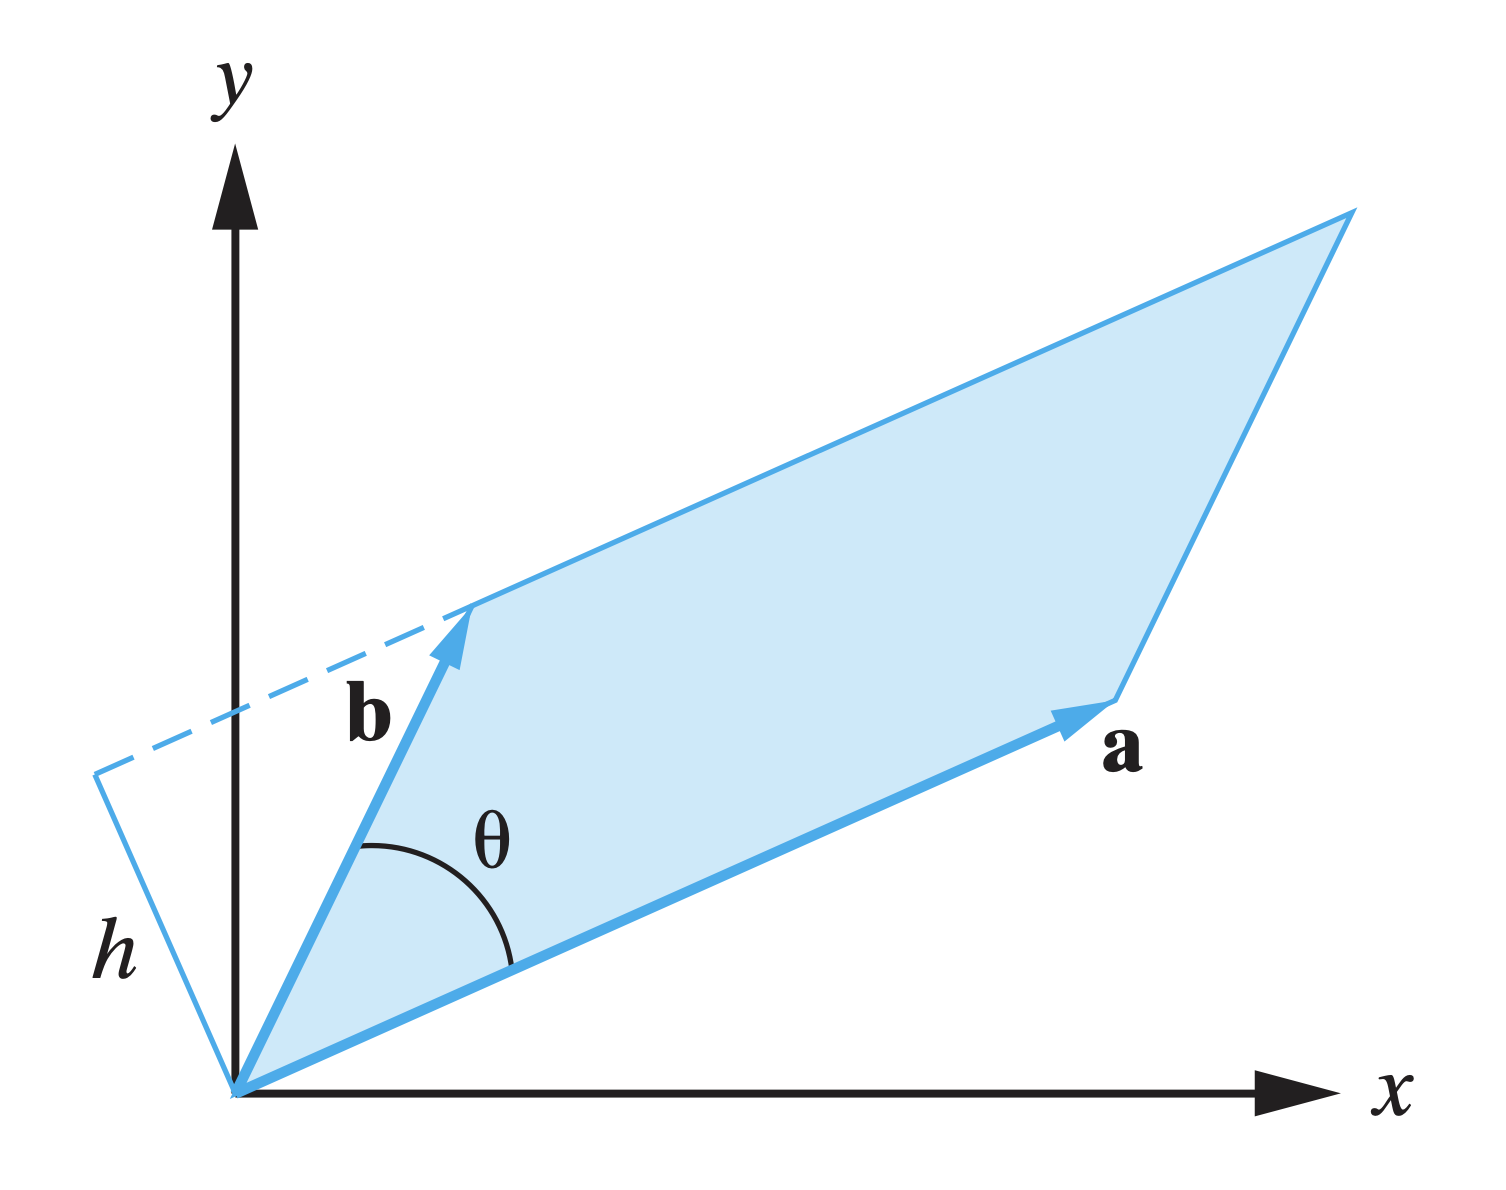
\includegraphics[scale=0.2]{img/Snipaste_2024-03-27_22-33-20.png}
        \caption{Area of a parallelogram}    
    \end{center}
\end{figure}




\ex{
    \textbf{Find the area of the triangle with vertices $(1,1), (2,3), (6,9)$.}
    \[
        \begin{vmatrix}
            1 & 1 \\
            2 & 3
        \end{vmatrix}
        = 1 \cdot 3 - 1 \cdot 2 = 3 - 2 = \boxed{1}
    \]
    Note: Since the vector $(6, 9)$ is a multiple of the vector $(2, 3)$ (linearly dependent), we can ignore the third vertex $(6, 9)$.

    



}
















\newpage

\section{Lecture 10: Rank, Invertibility, Elementary Row Operations \& additional properties of determinants}







% ------------------------------------------------------------------------------
\chapter{Vector Spaces}
\section{Lecture 11: Vector Spaces, Zero-Vectors, Dimentions, basis, \& Linear Combinations}



\newpage
\section{Lecture 12: Vector Subspace \& Proof}




\newpage
\section{Lecture 13: Spanning Set}




\newpage
\section{Lecture 14: Spanning, Linear Independence \& Basis}

\newpage
\section{Lecture 15: Linear Independence \& Basis and dimension}

\newpage
\section{Lecture 16: Basis, Row and Columns Spaces}































































\end{document}
